\newpage
\vskip 6mm
\pagestyle{myheadings}
\markboth{{\underline{\centerline{东南大学博士学位论文} }}}
{{\underline{\centerline{第一章 \ \ \  绪论} }}}
\chapter{绪论}\label{ch1}
\setcounter{equation}{0}
%\renewcommand{\theequation}{\thesection.\arabic{equation}}

\section{时滞复杂网络概述}\setcounter{equation}{0}
从生态系统到社会系统,从人际关系网到万维网,广泛存在于自然界和人类社会中的复杂系统都可以由相应的复杂网络模型刻画。复杂网络的数学理论来源于经典的图论 \cite{bondy1976graph},其发展经历了一个漫长的探索过程。
最早的研究始于 1736 年欧拉提出的柯尼斯堡七桥问题,但在之后相当长的一段时间都没有实质性进展。直到 20 世纪 60 年代,随机图理论 \cite{gilbert1959random1141} 的建立为网络构造提供了一种新的方法,正式开启了复杂网络的理论研究。随后, 在 20 世纪 90 年代,小世界网络\cite{watts1998collective440} 和无标度网络\cite{barabasi1999emergence509} 的提出打破了随机图理论的框架,开启了复杂网络研究的新纪元。在过去的几十年里,复杂网络已经成为众多学科争相关注的焦点,例如生物科学、计算机科学、物理科学、图论以及社会学等 \cite{dehmer2009analysis,costa2011analyzing329,estrada2012structure}。在实际的复杂网络中,由于信息传输和采样速度有限、网络带宽受限以及物理元件老化等原因,时滞往往是不可避免的,这导致系统当前的发展趋势不仅依赖于当前的状态,还依赖于过去的状态 \cite{xu2006epidemic525,liu2009structure1799,wang2015event2497}。 时滞的存在通常会导致复杂网络产生振荡、发散等不良性能。因此,时滞复杂网络的研究是非常有必要和有意义的。


在时滞复杂网络中,时滞可以分为耦合时滞 (即节点之间通讯产生的时滞) \cite{Lu2008Local,Fei2009New,Wang2010Chaos,Wu2013Sampled,Park2018Closeness,wang2011mixed,syed2019synchronisation585} 和状态时滞 (即节点自身信息反馈产生的时滞) \cite{liu2017partial3906,zou2015event2804};也可以分为常时滞和时变时滞。为了研究不同类型的时滞,不同的研究方法相继被提出。
最早的方法为频域法 (直接法) \cite{gu2003stability},通过分析系统的特征根在复平面上的分布来研究系统的动态性能。虽然这种方法更加直观形象且易于理解,但是对于具有大规模节点的复杂网络来说,其特征方程为超越方程,计算出所有的特征根是不切实际的。随后,时域法 (间接法) \cite{fridman2014introduction,sun2012timedelaystability} 被提出,它被广泛用于处理时变时滞系统、参数不确定的时滞系统和时滞非线性系统,是目前最主要的研究方法。 时域法主要有 Lyapunov-Krasovskii 泛函法 (充分利用时滞信息) 和 Lyapunov-Razumikhin 函数法 (不借助于时滞信息)。通常, Krasovskii 法被用于处理具有较小或变化缓慢的时滞的系统,提供依赖于时滞的条件;而 Razumikhin 法则被用于处理具有较大或变化比较快的时滞的系统,提供不依赖于时滞的条件。

 网络拓扑结构是时滞复杂网络的重要组成部分,可以清楚地反映网络节点之间的连接关系,即节点之间的信息交流 \cite{wang2002complex885}。起初,时滞复杂网络的网络拓扑主要设定为节点间的拓扑关系不随时间发生改变且网络中的所有边都是无方向的,此时网络具有无向的静态 (固定) 拓扑结构 \cite{cheng2013mean261}。 而现实世界中大多数网络,例如电网、食物链网络和引文网络等都是有向的 \cite{camacho2002robust, yu2009second881,gu2019pidDOI}。此外,
随着空间和时间的推移,网络的节点数可能会不断地增加或减少,并且节点之间的权重和连接方式都可能是动态变化的,这导致网络拓扑是不断发生变化的。例如无线传感器网络中节点可能出现移动、故障等情况,万维网的网页随时可能出现或断开。因此,具有有向动态网络的时滞复杂网络吸引了大量研究者的关注,其中切换拓扑作为动态网络结构中比较重要的类型已有大量相关结果被提出并发表 \cite{wang2011synchronization3070,jin2015function730,chen2016synchronizing189,li2017state6377}。
\section{时滞复杂网络动力学的研究背景及现状}
由于时滞复杂网络中不同的网络拓扑、每个子系统的非线性以及时滞的存在,使时滞复杂网络在演化过程中能够产生丰富的动力学行为。 
\subsection{同步的研究背景及现状} 
同步作为一种重要的集群行为,广泛存在于自然界、工程和社会生活中,例如钟摆的同步摆动,
成千上万的萤火虫以共同的频率发出光脉冲,人体大脑神经网络和心脏肌肉细胞的共同振动,管弦乐队中小提琴手们齐声演奏等 \cite{mirollo1990synchronization1645,fries2001modulation1560,steinmetz2000attention187}。在过去的十几年里,时滞复杂网络的同步问题吸引了众多国内外学者的关注且收获颇丰。
其中,
完全同步是形式最简单也是研究最多的同步类型,是指在不同的初始条件下两个或多个动力系统,通过动力系统间的相互作用,使得各个动力系统状态逐渐趋同,最终达到完全相同,其数学定义如下:
\begin{definition}  \cite{2018dynamicstimedelays}  记时滞复杂网络中节点 $i$ 的状态变量为 $x_i(t)$,$i\in I[1,N]$,如果 
\begin{align*}
\lim_{t\rightarrow \infty}|x_j(t)-x_i(t)|=0 
\end{align*}
对所有 $i$、$j\in I[1,N]$ 成立,那么,称时滞复杂网络可以实现完全同步。
\end{definition}  

 称 $\mathcal{S}=\{x=(x^T_1,x^T_2,\cdots,x^T_N)^T:x_1(t)=x_2(t)=\cdots=x_N(t)=s(t)\}$ 为时滞复杂网络状态控制中的同步流形,其中 $s(t)$ 是时滞复杂网络中孤立节点的解。那么,上述定义可以重新描述为: 
\begin{definition}   记时滞复杂网络中节点 $i$ 的状态变量为 $x_i(t)$,$i\in I[1,N]$,如果 
    \begin{align*}
    \lim_{t\rightarrow \infty}|x_i(t)-s(t)|=0 
    \end{align*}
    对所有 $i \in I[1,N]$ 成立。那么,称时滞复杂网络可以实现完全同步。
\end{definition}

近十几年来,众多学者从不同的方面、不同角度对时滞复杂网络的完全同步进行了研究 \cite{liang2008exponential153,song2012global2389,shi2016synchronization178,zhang2008adaptive183,stilwell2006sufficient140,hu2021sampled3071811,2019Adaptively2943621,liu2007exponential82,yang2015robust1077,wu2015exponential3097,popov2012robust2343,wang2013robust2097}。%通信时滞;状态时滞;时滞;常时滞;时变时滞;无穷时滞(比例时滞)
从时滞的角度来看,
借助 Lyapunov 方法和随机分析技术,song 等人研究了具有状态和耦合常时滞的复杂网络的完全同步问题 \cite{song2012global2389},得到了依赖于时滞的同步判据。在此基础上,Shi 等人通过设计合适的控制协议进一步讨论了具有时变时滞的复杂网络完全同步问题 \cite{shi2016synchronization178}。最近,Tang 等人将有界时滞的结果推广到无穷时滞, 研究了自适应策略下具有无穷时滞的复杂网络的完全同步问题 \cite{2019Adaptively2943621}。
%固定拓扑;切换拓扑;时变拓扑;
从网络拓扑的角度来看,前期的研究结果主要集中于具有固定拓扑的时滞复杂网络。然而,在网络的实际演化过程中,由于节点的增多或减少以及网络问题等原因,网络拓扑结构总是不断变化的,并且时变的网络拓扑可以传输更多的网络信息。因此,时变的网络拓扑越来越受到人们的关注,例如,具有时变网络拓扑的时滞复杂网络的完全同步问题在文献 \cite{stilwell2006sufficient140,popov2012robust2343} 中进行了研究,为网络拓扑时变时的完全同步提供了新的见解。此外,作为时变网络拓扑的最为常见的类型,具有切换拓扑的时滞复杂网络的完全同步也被充分讨论 \cite{hu2021sampled3071811,wang2013robust2097}。研究表明,网络拓扑结构对时滞复杂网络同步性能有着显著的影响。 %%%非线性耦合
从不同类型的耦合项来看,大部分的完全同步结果都集中于具有线性耦合项的时滞复杂网络。 而在现实的网络中,节点的邻居信息在绝大多数情况下无法实时获得,那么存在邻居节点未知但是满足非线性函数的情况,因此具有非线性耦合项的时滞复杂网络得到了关注,相应的完全同步准则也被提出 \cite{liu2007exponential82,yang2015robust1077,wu2015exponential3097}。

时滞复杂网络的完全同步实际上是比较理想的情况,而现实的时滞复杂网络的动力学可能是非常复杂的,完全同步可能无法实现,尤其是节点存在不同的动力学特征。因此,其他形式的有序行为,例如相位同步、集群同步、投影同步等广义同步被相继提出,并且越来越受到关注 \cite{2009The1276,2013Function1182,Zhi2017Cluster585,wang2018generalized6597,chen2021quasi3103597,lu2019phase122419,han2016modified1650126}。例如,大规模时滞复杂网络的相位同步在文献 \cite{2009The1276,lu2019phase122419} 中被讨论,从能量的角度观察和分析网络的相位同步而振幅可以相关很差或没有关联。大多数情况下,投影同步都是将系统的状态同步到给定的常数比例因子,而文献 \cite{2013Function1182,han2016modified1650126} 改进了这一结果,研究了时滞复杂网络的函数投影同步,其中比例因子是函数比例因子。随后,为揭示耦合基因振荡器网络不同集群规律行为的产生机制,Guan 等人分析了时滞耦合基因调控网络的集群同步
\cite{Zhi2017Cluster585},描绘了在同一集群中的节点可以实现完全同步,在不同集群中的节点无法实现同步的动力学行为。 最近,通过设计基于离散时间状态观测的非周期间歇控制协议,Chen 等人 
研究了模糊异构的复杂网络的拟同步,描绘了具有不同动力学的节点之间存在有界误差的动力学行为 \cite{chen2021quasi3103597}。为了描述更多丰富的有序行为,时滞复杂网络的广义同步还值得进一步探索与研究。 
\subsection{一致性的研究背景及现状}
一致性是复杂网络除同步外又一重要而特殊的动力学行为,主要用于描述为满足工程需求而提出的结构更加简单的分布式多智能体系统。所谓一致性是指多智能体系统中的个体在局部协作和相互通信下,随时间的演化 最终使得所有智能体在某个目标量上趋于一致,描述了智能体之间相互作用、传递信息的过程。在过去的十几年,多智能体系统的一致性问题已被广泛应用在无人机编队控制、交通车辆控制、网络的资源分配等众多领域,成为当前工程领域研究的热点 \cite{2011DistributedLondon,2013An427,2018Multi345}。一致性的数学定义有以下两种:
\begin{definition} \cite{gao2018xuconsensus}(\textbf{领导者--跟随一致性})  假设多智能体系统中有 $N+1$ 个智能体,记第 $i$ 个智能体的状态变量为   $x_i(t)$,$i\in I[0,N]$,如果 
    \begin{align*}
    \lim_{t\rightarrow \infty}|x_i(t)-x_0(t)|=0
    \end{align*}
    对所有 $i\in I[0,N]$ 成立,则称多智能体系统达到状态一致。其中,智能体 $0$ 被称作是领导者, 其他的智能体 $i$,$i\in I[1,N]$ 被称作是跟随者。
\end{definition}   
\begin{definition} 
    \cite{gao2018xuconsensus}(\textbf{无领导者一致性}) 假设多智能体系统中有 $N$ 个智能体,记第 $i$ 个智能体的状态变量为 $x_i(t)$,$i\in I[1,N]$,如果 
    \begin{align*}
    \lim_{t\rightarrow \infty}|x_j(t)-x_i(t)|=0,\ \forall i\neq j 
    \end{align*}
    对所有 $i$、$j\in I[1,N]$ 成立,则称多智能体系统达到一致性。
\end{definition}
 
 现实的网络环境是复杂多变的,多智能体系统在实际运行中普遍具有非线性特性和时滞。因此,非线性时滞多智能体系统的一致性问题受到越来越多的关注 \cite{2015Sampled369,2016Consensus3311,2014Adaptive1217,2020Quasi2964826}。 相比时滞复杂网络的同步,非线性时滞多智能体系统的一致性则更强调智能体之间的局部信息的交流方式。近几年来,国内外的大量学者沿着不同的思路和方法对非线性时滞多智能体的一致性从多个方面进行了深入研究,不同的一致性算法被开发。 

\textbf{领导者--跟随一致性}  
在带有领导者的非线性时滞多智能体系统中,领导者代表着跟随者共同跟踪的目标或者整个系统的共同利益,通过对跟随者设计合适的控制协议,使得领导者和跟随者的最终状态达到一致。目前,带有领导者的一致性主要包括单个领导者的一致性和多个领导者的一致性 \cite{2015Event1998,2011Output200,2017A1625,2021Leader109444,wang2022leader127031,yue2019neuro230,li2021distributed109545,wen2020fault}。
对于具有单个领导者的非线性时滞多智能体系统,通过设计连续的反馈控制器,非线性时滞多智能体系统的领导者--跟随一致性问题在文献  \cite{2011Output200,2017A1625,2021Leader109444,wen2020fault} 中被充分讨论。而通过设计不连续的分布式脉冲控制策略,
文献 \cite{wang2022leader127031,wen2020fault} 提出了不连续的分布式脉冲牵制控制策略,分别研究了具有时变时滞和分布式时滞的非线性多智能体系统的领导者--跟随一致性。当领导者具有高维的动态且无法进行测量时,Yue 等人讨论了非线性时滞多智能体系统一致性跟踪问题 \cite{yue2019neuro230} 。
当具有多个领导者时,Li 等人利用分布式自适应输出反馈控制器解决了不确定的非线性时滞多智能体系统包围控制问题\cite{li2021distributed109545},此时跟随者的状态最终渐近收敛到领导者所形成的凸包内。

\textbf{切换拓扑下一致性}  在非线性时滞多智能体系统的运行过程中,由于移动的智能体超出彼此的有效检测范围,或者移动的智能体存在未知障碍物等原因,智能体之间的通信链路可能发生变化 (中断或增加),这意味着网络拓扑是动态变化的 \cite{jiang2020non210,li2018data1773,yaghoubi2020cluster1685,jiang2021h280,li2013second1595}。其中,切换拓扑是最重要也是研究最多的动态拓扑, Jiang 等人讨论了在采样控制下具有切换拓扑非线性时滞多智能体系统的非脆弱 H$_\infty$ 一致性跟踪问题 \cite{jiang2020non210} 。Li 等人  通过设计分布式数据驱动的一致性协议分析了具有切换拓扑的非线性时滞多智能体系统的输出一致性 \cite{li2018data1773}。基于脉冲控制,Yaghoubi 等人研究了具有切换拓扑的分数阶非线性时滞多智能体系统的集群一致性  \cite{yaghoubi2020cluster1685}。特别地,当网络拓扑是随机切换时, 具有马尔可夫切换拓扑的非线性时滞多智能体系统的一致性问题在文献 
\cite{jiang2021h280,li2013second1595} 中被讨论,其中网络拓扑之间服从马尔可夫过程,马尔可夫过程的状态空间相当于所有可能的拓扑。

 
\textbf{具有通信时滞一致性} 由于智能体之间的传输速度受限以及通道带宽有限等原因, 多智能体系统不可避免地存在通讯时滞。通常,通信时滞的存在会降低多智能体系统的系统性能甚至导致系统的不稳定。因此,研究具有通信时滞的多智能体的一致性是非常有必要的。近年来,具有通信时滞的非线性多智能体系统的一致性得到了研究者们极大的关注,一些有趣的结果被相继提出 \cite{sharifi2020finite10,2019Leader,2021Consensus126,lu2019consensus153,wang2016distributed918}。 例如,Sharifi 等人研究了在混合连续控制下具有通信常时滞的非线性多智能体系统的有限时间一致性问题   \cite{sharifi2020finite10}。通过设计可靠控制器, Subramanian 等人分析了具有时变通信时滞的一阶非线性多智能体系统领导者--跟随一致性问题  \cite{2019Leader}。
Jiang 等人通过引入非周期性数据采样控制机制,研究了具有通信时滞的高阶非线性多智能体系统一致性追踪问题 \cite{2021Consensus126}。 当网络拓扑图是具有拮抗作用的符号图时,Lu 等人研究了具有不同的通信时滞的非线性多智能体系统的二部一致性问题 \cite{lu2019consensus153,wang2016distributed918}。

\textbf{局部一致性}
目前,许多研究人员已经对非线性时滞多智能体系统进行了大量研究,但不难发现, 大多数一致性的理论结果都是 建立在理想通信条件下且要求智能体的非线性项满足全局 Lipschitz 条件,因此所得都是全局一致性结果,这些全局性的假设具有一定的局限性和保守性。 因此,近几年非线性时滞多智能体系统的局部一致性得到关注 \cite{qian2017local2462,2019dynamic1699}。
为了避免全局 Lipschitz 假设带来的保守性,Qian 等人通过定义智能体的加权平均状态并应用局部线性化研究了非线性时滞多智能体的局部一致性 \cite{qian2017local2462}。
此外,当执行器达到饱和时, 一致性无法对多智能体系统的所有初值都实现,只能在有界初值下才能实现。Liu 等人
 研究了非线性时滞多智能体系统的局部一致性并设计优化算法估计出吸引域 \cite{2019dynamic1699}。
目前,对非线性时滞多智能体的局部一致性分析还较少,值得进一步深入研究。
\section{脉冲控制的研究背景及现状}\setcounter{equation}{0}
\subsection{脉冲控制的研究背景}
20 世纪 90 年代,随着脉冲微分方程理论在控制领域中应用的不断深入以及工业上越来越多的元件以脉冲微分方程建模,例如捕食者--食饵系统、混沌扩频系统和纳米电子器件等,脉冲控制系统引起了数学家、物理学家以及工程师的极大兴趣,并获得了突飞猛进的发展 \cite{lakshmikantham1989theory}。随后,脉冲控制的基本框架被提出 \cite{yang2001impulsive},不同于连续的控制方法,脉冲控制仅通过瞬时改变系统的状态就能达到控制效果,为控制领域提供一种全新的控制策略,其定义如下:
\begin{definition} \cite{yang2001impulsive}
 给定一个 状态变量为 $z\in\mathbb{R}^n$ 的非脉冲的机构 $\mathcal{P}$,控制时间序列 $T=\{t_k\}$,$t_k\in\mathbb{R}$,$t_k<t_{k+1}$,$k\in\mathbb{Z}_+ $ 和控制律 $\mathcal{I} (k,x)\in\mathbb{R}^n$,如果在每个脉冲时刻 $t_k$,状态变量 $z$ 被瞬时改变为 $z(t_k)=z(t^-_k)+ \mathcal{I} (k,z)$,使得当 $t\rightarrow \infty$ 时,系统的输出 $y=g(t,z)$,$g: \in\mathbb{R}_+\times \mathbb{R}^n\rightarrow \mathbb{R}^m$,$ y\in\mathbb{R}^m$ 逼近目标 $y^*\in\mathbb{R}^m$,该控制方法被称为脉冲控制。
\end{definition} 
其中,机构 $\mathcal{P}$ 中至少有一个状态变量被瞬时改变为控制律给定的任意值,这意味着并不是机构 $\mathcal{P}$ 中所有的物理系统都能被施加脉冲控制,也可能同时受到非脉冲控制。另一方面,脉冲控制的时间序列 $\{t_k\}$,$k\in\mathbb{Z}_+$ 可以是周期的,也可以非周期的。

脉冲控制的数学基础是脉冲微分方程,根据脉冲发生的不同特征,主要有以下三种类型:

\textbf{(1) 脉冲控制发生在固定时刻} 脉冲控制发生在时间序列 $\{t_k\},\  k\in\mathbb{Z}_+$ 上,即所谓的依赖于时间的脉冲控制, 其脉冲微分方程可以写成 
\begin{align*} \left\{
\begin{aligned} 
&\dot{z}(t)=f(t,z(t)),\ t\neq t_k,\ k\in \mathbb{Z}_+,\\
&\Delta z(t_k)=\mathcal{I}_k (z(t^-_k)),  
\end{aligned}
\right.
\end{align*}
其中 $\Delta z(t_k)=z_i(t_k)-z_i(t^-_k)$,$ z_i(t^-_k)=\lim_{t\rightarrow t^-_k}z_i(t_k)$, $z_i(t_k)=z_i(t^+_k)=\lim_{t\rightarrow t^+_k}z_i(t_k)$。

\textbf{(2) 脉冲控制发生在可变时刻}  \cite{yang2017synchronization115} 当系统的轨迹撞击增广相空间的超曲面  
$\mathcal{H}(t,z)=0$
时,产生脉冲控制,即所谓的依赖于状态的脉冲控制,其脉冲微分方程可以写成 
\begin{align*} \left\{
\begin{aligned} 
&\dot{z}=f(t,z ),\ \mathcal{H}(t,z)\neq 0,\\
&\Delta z =\mathcal{I}(z(\tau_k(x))),\ \mathcal{H}(t,z)=0.
\end{aligned}
\right.
\end{align*}
在不同初始条件下,该类系统的解具有不同的脉冲点。在这种情况下,系统的一个解可能会撞击同一个超曲面很多次,导致脉动现象。另一方面,系统的不同的解也可能在一段时间后重合,并在此后表现为单一的解,从而导致解的合并。因此,该类脉冲控制的研究比发生在固定时刻的脉冲控制更加困难。
 
\textbf{(3) 自治的脉冲控制} \cite{goedel2012hybrid}  这类系统的状态不依赖于时间 $t$,脉冲的发生依赖于系统的状态,其脉冲微分方程可以写成
\begin{align*} \left\{
\begin{aligned} 
&\dot{z} =f(z),\ z\notin \mathcal{S},\\
&\Delta z =\mathcal{I}(z),\  z\in \mathcal{S}.
\end{aligned}
\right.
\end{align*}
 
 
脉冲控制作为一种强大的不连续控制方法,受到了大多数研究人员的青睐,因为它仅在某些离散时刻改变系统的状态就能达到控制效果 \cite{2020Synchronization38,tang2015leader346}。与状态反馈控制等连续控制方法相比,瞬时的脉冲跳变增强了对外部干扰的鲁棒性,并能有效减少信息传输量。因此,脉冲控制具有成本更低、效率更高、鲁棒性更强、保密性更好等优点。 
\subsection{脉冲控制的研究现状}
在过去的几十年里,脉冲控制已经被广泛应用于各种领域,例如市场中货币供用控制、深空航天器轨道修正、房室模型中静脉给药治疗以及通信保密等 \cite{haddad2006impulsive,goedel2012hybrid}。因而,脉冲控制得到国内外学者的广泛重视,大量的研究成果被报道 \cite{yang1997impulsive645,lu2010unified1215,wang2018unified25,lu2012pinning1250176,sun2012outer1751,feng2016exponential621}。其中,Yang 等人通过脉冲控制研究了非线性动态系统的渐近同步并提出一种新的混沌通信方案 \cite{yang1997impulsive645},并给出了脉冲间隔的上界的估计。随后,Lu 等人提出了平均脉冲区间的概念, 消除了对脉冲间隔上下界的限制, 在脉冲控制下解决了复杂网络的同步问题 \cite{lu2010unified1215}。对于脉冲控制下的时滞复杂网路的同步问题, 借助于脉冲时滞系统的比较原理,时滞复杂网络指数同步问题在文献 \cite{lu2012pinning1250176,sun2012outer1751} 中被讨论,但是它们对于脉冲间隔的上下界都有严格的限制。Feng 等人则取消了这一限制,利用平均脉冲区间的方法,讨论了脉冲控制下具有状态时滞和耦合时滞的复杂网络指数同步问题 \cite{feng2016exponential621},允许非均匀分布的脉冲控制信号的存在。
  

近几年来,随着对脉冲控制研究的逐渐深入,许多专家不再满足传统的脉冲控制,不同类型的脉冲控制相继被提出,并被推广到时滞复杂网络的动力学分析中,主要包括下面几种类型:


 \textbf{ 时滞脉冲}  在实际操作过程中,由于频繁的数据采样导致的数据包冲突会造成丢包,这意味着脉冲控制中的瞬时跳变不仅取决于系统的当前状态,还取决于过去的状态,即时滞脉冲控制。在现实控制系统中,时滞脉冲控制广泛应用于股市市场
 、病虫害的防治、疫苗的脉冲免疫接种等,越来越多的学者们加入到对时滞脉冲控制的研究中来,许多重要的成果被报道 \cite{liu2018consensus134,Li2016Stabilization,Zhang2015Synchronizationof,Li2016Stability,He2017Network,Yang2018Review,he2020synchronization}。通常情况下,时滞的存在会降低脉冲控制器的控制性能。 
 利用拓展的 Halanay 不等式和新型的脉冲微分方程, Zhang 等人  讨论了时滞脉冲控制下基于忆阻器的耦合时滞递归神经网络的同步问题 \cite{Zhang2015Synchronizationof}。基于分布式时滞脉冲控制,非线性多智能体系统的领导者--跟随一致性问题在文献 \cite{He2017Network} 得到解决。 另一方面,脉冲控制中时滞信号的存在可以促进系统的稳定性甚至镇定不稳定的系统。例如,Li等人利用脉冲时滞不等式研究了时滞系统的指数镇定性 \cite{Li2016Stabilization} , 该研究成果充分考虑
了脉冲中时滞的有益影响。受此启发,基于 Lyapunov 方法和平均脉冲区间的方法,He 等人讨论了时滞脉冲控制下复杂网络的全局指数同步问题 \cite{he2020synchronization},其中脉冲控制中的时滞的镇定作用被充分考虑。因此,脉冲控制中的时滞对复杂网络的动态性能具有两面性。

\textbf{ 牵制脉冲}   传统的脉冲控制需要在脉冲时刻对网络中所有的节点施加控制,但是当网络规模比较大的时候,不可能控制网络中的每一个节点,这是非常昂贵且不切实际的。为了解决这个问题,牵制脉冲控制策略被提出,其在脉冲控制的基础上进一步考虑了牵制控制,本质上是仅对大规模网络中的部分关键节点施加脉冲控制,通过节点之间的相互耦合影响网络中的其它节点,从而达到控制整个网络的目的。由于可以节约更多的网络资源,牵制脉冲控制更适合节点较多的复杂网络,被广泛用于解决时滞复杂网络的同步问题 \cite{2012Synchronization285,2013Synchronization3486,2019An2561,zhou2011pinning2882,liu2020intralayer3006032}。  通过牵制脉冲控制,Yang 等人讨论了具有时变时滞的耦合的反应--扩散神经网络的同步问题 \cite{2013Synchronization3486}。随后,Wang 等人
提出了具有记忆功能的牵制脉冲控制方法,分析了具有参数不匹配和时变时滞的复杂网络的集群同步问题 \cite{2019An2561}。特别地,Zhou 等人考虑仅对网络中的单个节点施加脉冲控制 ,设计了牵制的单个脉冲控制策略,验证了只要正确选择网络的耦合强度和耦合时滞,牵制的单个脉冲控制仍然可以保证时滞复杂网络的同步 \cite{zhou2011pinning2882}。 

\textbf{混杂脉冲控制} 由于传统的脉冲控制仅在离散时刻发挥作用,而在脉冲间隔内没有任何控制行为,为了获得更好的收敛性能,在脉冲控制间隔内进一步施加连续的控制,即混杂脉冲控制。这种控制方法同时拥有脉冲控制和连续控制的优点。尤其适用于其中一种控制效果不佳甚至失效,另一种控制仍然会使系统达到所期望的控制效果。因此,混杂脉冲控制比单个控制方法具有控制性能更高、鲁棒性更强的优点。近几年,混杂脉冲控制被广泛用于时滞复杂网络的同步的研究 \cite{yang2014hybrid480,2020Synchronization4043,li2019global31}。例如,通过设计包含自适应控制和脉冲控制的混杂脉冲控制策略,文献 \cite{yang2014hybrid480}  研究了
具有不确定扰动的时滞复杂网络同步问题。Yang 等人文献同时考虑了脉冲控制和执行器故障反馈控制,并在此混杂脉冲控制器下分析了具有切换拓扑的时滞复杂网络的几乎必然全局指数同步问题 \cite{2020Synchronization4043}。Li 等人  利用包括连续时间状态反馈控制和脉冲控制的混杂脉冲控制策略,讨论了具有耦合时滞的分数阶复杂网络的全局同步控制问题\cite{li2019global31}。



 \textbf{事件触发脉冲控制} 
为了降低与连续控制的偏差、确保控制性能,脉冲控制都需要频繁的采样频率。这意味着不管系统性能有无明显变化,脉冲控制都需要以固定的频率 (基于时间触发) 进行信息传输和控制更新,故不再适应于大规模的复杂网络。最近,资源利用率更高的控制方法——事件触发脉冲控制被提出,主要思想是将脉冲控制考虑到事件触发机制中。不同于传统的脉冲控制和事件触发控制,事件触发脉冲控制仅在系统的性能指标超出一定阈值时才更新脉冲控制信号,并且在触发的时间间隔内不执行任何控制指令,这极大地减少了发送的数据包数量,节约了通信资源,减少了网络问题对系统性能和稳定性的负面影响。近年来,一些有关事件触发脉冲控制的结果被提出 \cite{2019Consensus792,Zhu2018Event,2020Leader1,2021Synchronization2491}。例如,Zhu 等人借助事件触发脉冲控制研究了连续时间动态系统的指数稳定并将结果推广到忆阻神经网络的同步 \cite{Zhu2018Event}。基于分布式事件触发的脉冲控制,Tan 等人研究了多智能体系统的一致性问题 \cite{2019Consensus792}。 
最近,Hai 等人进一步将牵制控制和事件触发的脉冲控制相结合,提出了事件触发的牵制脉冲控制策略  \cite{Xudong2020Pinning105017},讨论了分数阶时滞复杂网络的同步问题。 尽管事件触发脉冲控制优势明显,但也会导致时滞复杂系统呈现更复杂的不连续行为,因而分析与设计更具挑战性。

 
 \textbf{饱和脉冲控制}    在许多实际控制系统中,执行器饱和是不断发生的,这源于系统的物理特性的限制和安全运行的需求 \cite{brieger2009flight92,farantatos2015predictive1826,xiao2011adaptive1605}。当执行器达到饱和,如果输入较大的控制信号,执行器只能传输具有幅度或速率限制的信号,这就导致控制器状态被错误更新从而降低系统的控制性能。因此,在设计脉冲控制方法时充分考虑执行器饱和是非常有必要的。实际上,饱和脉冲系统在真实网络中广泛存在,例如工业污水处理系统、汽车操纵系统等。近年来,具有执行饱和的脉冲控制得到了关注,但是由于脉冲饱和项难处理以及吸引域难于估计,关于饱和脉冲控制下复杂网络的研究工作甚少,尚还处于起步阶段 
 \cite{li2020impulsive,li2020impulsivePolytopic,2019dynamic1699,shen2019estimation,HE2021126452,ouyang2020impulsive}。例如,通过设计饱和脉冲控制器,Li 等人文献研究了耦合的时滞神经网络的同步问题  \cite{ouyang2020impulsive},并将所得结果应用到图像加密中。
从现有的饱和脉冲的结果中不难发现, 收缩的不变集被普遍应用于吸引域的估计,因为它具有所有从集合出发的状态轨迹始终保持在其内部并最终收敛到原点的性质。也就是说系统的 Lyapunov 能量函数是单调递减的,这意味着利用收缩的不变集来估计吸引域对具有饱和脉冲控制的系统来说具有保守性。目前,迫切需要探索一种新的估计吸引域的方法。
\section{预备知识}
\subsection{代数图理论}
$\mathcal{G}=(\mathcal{V},\mathcal{E})$ 表示 $N$ 阶有向图,其中 $\mathcal{V}=\{v_i$,$i\in I[1,N]\}$ 为顶点集,  $\mathcal{E}\subseteq\mathcal{V}\times\mathcal{V}$ 为边集。有向图 $\mathcal{G}$ 中的边 $\mathcal{E}_{ij}$ 可由有序对 $ (v_i,v_j)$,$i$、$j\in I[1,N] $ 表示,其中 $v_i$ 为起点,  $v_j$ 为终点,这意味着节点 $v_j$ 可以接收来自节点 $v_i$ 的信息,$v_i$ 被称为父节点, $v_j$ 被称为子节点。
节点 $v_i$ 的邻居可记为 $\mathcal{N}_i=\{v_j\in \mathcal{V}|(v_j,v_i)\in\mathcal{E}\}$。图 $\mathcal{G}$ 中从节点 $v_i$ 到节点 $v_j$ 的有向路径是有向边序列 $(v_{i_1},v_{i_2})$,$(v_{i_2},v_{i_3})$,$\cdots$,$(v_{i_{m-1}},v_{i_m})$,其中 $v_i=v_{i_1}$,$v_j=v_{i_m}$。
如果存在一个节点 $v_r$,使得对于其他任意节点 $v_s\in\mathcal{V}$,都存在一条从 $v_r$ 到 $v_s$ 的有向路径,那么就称 $\mathcal{G}$ 包含有向生成树。
如果任意两个节点之间都存在有向路径,则此有向图 $\mathcal{G}$ 是强连通的。

有向图 $\mathcal{G}$ 的邻接矩阵 $\mathcal{A}=[a_{ij}]_{N\times N}$ 定义为 $a_{ij}>0$ 当且仅当 $(v_j,v_i)\in\mathcal{E}$,且对所有的 $ i\in I[1,N]$ 有 $a_{ii}=0$。拉普拉斯 
矩阵 $\mathcal{L}=[l_{ij}]_{N\times N}$ 定义为 $\mathcal{L}=\mathcal{D}-\mathcal{A},$ 其中 $\mathcal{D}={\rm diag}\{d_1,d_2,\cdots,d_N\}$ 是度矩阵,且元素 
$d_i=\sum\limits_{j\in \mathcal{N}_i}a_{ij}$ 为节点 $v_i$ 的入度。  对于由 $N$ 个跟随者和一个领导者组成的多智能体系统,网络拓扑由有向图 $\bar{\mathcal{G}}$ 表示,其由有向图 $\mathcal{G}$ 和节点 $v_0$ 构成。定义 $\mathcal{H}=\mathcal{L}+\mathcal{B}$, 其中 $\mathcal{B}={\rm diag}\{b_1,b_2,\cdots,b_N\}$,如果领导者 $v_0$ 是跟随者 $v_i$ 的邻居,则 $b_i>0$,否则 $b_{i}=0$。
\begin{definition} \cite{2011DistributedLondon} 
设矩阵 $A\in\mathbb{R}^{N\times N}$,$N\geq 2$,若存在置换矩阵 $P\in\mathbb{R}^{N\times N}$,使得
 \begin{align*}P^T AP=
\left[ \begin{array}{cc } 
A_{11} & \mathbb{O}_{k\times (N-k)}\\
A_{21} &A_{22}
\end{array}\right], 
\end{align*}
其中 $A_{11}\in\mathbb{R}^{k\times k}$,$A_{21}\in\mathbb{R}^{(N-k)\times k}$, $A_{22}\in\mathbb{R}^{(N-k)\times (N-k)}\ (1\leq k\leq N-1)$,则称矩阵 $A$ 是可约的;否则,称矩阵 $A$ 是不可约的。 
\end{definition} 

\begin{lemma} \cite{lu2006new214}\label{l1-3-1}
    假设 $A=[\tilde{a}_{ij}]_{i,j=1}^{N}\in \mathbb{R}^{N\times N}$, 如果
    \begin{description}
        \item $(1)$ $\tilde{a}_{ij}\geq 0$,$i\neq j$,$ \tilde{a}_{ii}=-\sum\limits_{j=1,j\neq i}^{N}\tilde{a}_{ij}$,$i\in I[1,N]$;
        \item $(2)$ $A$ 是不可约的,
    \end{description}
    那么下式成立:
\begin{description}
\item $(a)$   ${\rm rank}(A)=N-1$,即 $0$ 是 $A$ 代数几何重数为 $1$ 的特征值,且 $A$ 的所有非零特征值均有负实部;  
\item $(b)$ 假设 $\xi=(\xi_1,\xi_2,\ldots,\xi_N)^T\in\mathbb{R}^{N}$ (不失一般性,假设 $\sum\limits_{i=1}^{N}\xi_i=1)$ 是矩阵 $A$ 特征值等于 $0$ 所对应的左特征向量。那么 $\xi_i>0$, $\forall i\in I[1,N]$。令 $\xi_{\max}=\max\{\xi_i\}$,$ \xi_{\min}=\min\{\xi_i\}$;
\item $(c)$ 令 $\Xi={\rm diag}\{\xi_1,\xi_2,\ldots,\xi_N\}$,那么  $\tilde{A}=\Xi A+A^T \Xi$ 是一个对称矩阵,使得所有特征值都是实数并且满足  $0=\lambda_1(\tilde{A})>\lambda_2(\tilde{A})\geq\cdots\geq\lambda_N(\tilde{A})$。
    \end{description}
\end{lemma} 
\begin{lemma} \cite{yu2009second881}\label{l1-3-2}
    如果有向图 $\mathcal{G}$ 是强连通的,其拉普拉斯矩阵 $\mathcal{L}$ 特征值等于 $0$ 所对应的左特征向量为 $\tilde{\xi}=(\tilde{\xi}_1,\tilde{\xi}_2,\ldots,\tilde{\xi}_N)^T$,不失一般性,假设 $\sum\limits_{i=1}^{N}\tilde{\xi}_i=1$,那么存在正定对角矩阵 $ \Xi={\rm diag}\{\tilde{\xi}_1,\tilde{\xi}_2,\cdots,\tilde{\xi}_N\}$,使得  $\breve{\mathcal{ L}}=1/2( \Xi \mathcal{ L}+ \mathcal{ L}^T \Xi)$ 是对称矩阵,且 $\sum\limits_{j=1}^{N}\breve{l}_{ij}=\sum\limits_{i=1}^{N}\breve{l}_{ij}=0$,$ \forall i$、$j\in I[1,N]$。 
\end{lemma} 
\begin{definition} \cite{godsil2001algebraic} 
考虑强连通图 $\mathcal{G}$ 的拉普拉斯矩阵 $\mathcal{L}$,
代数连通度被定义为  \begin{align*}\lambda_\mu(\mathcal{L})=\min\limits_{x^T \xi=0, x\neq0}\dfrac{x^T\breve{\mathcal{L}}\chi}{ x^T \Xi x}.  
 \end{align*}
\end{definition} 
\begin{lemma}\cite{2015Event1998}  \label{l1-3-3}
有向图 $\bar{\mathcal{G}}$  包含有向生成树,其根节点为领导节点 $v_0$,则 $\mathcal{H}$ 的非对角项是非正的,并且其所有特征值都具有正实部。 
\end{lemma}
\subsection{矩阵理论} 
\begin{definition}设 $A=(a_{ij})_{m\times n},\ B=(b_{ij})_{p\times q}$,则 $A$ 和 $B$ 的 Kronecker  积是一个 $mp\times nq$ 的分块矩阵:
    \begin{align*}A\otimes B=
    \left[ \begin{array}{ccccc} 
    a_{11}B &a_{12}B&\cdots& a_{1n}B\\
    a_{21}B &a_{22}B&\cdots&  a_{2n}B\\
    \vdots&\vdots&\ddots&\vdots\\
    a_{m1}B &a_{m2}B&\cdots&  a_{mn}B
    \end{array}\right]. 
    \end{align*}
\end{definition}

\begin{lemma} \cite{horn2012matrix}\label{l1-3-4}
假设矩阵 $A$、$B$、$C$ 和 $D$ 具有适合维数,则有下列性质:
\begin{itemize}
    \item [$(1)$] 设 $k$ 为常数, 则有 $k(A\otimes B)=(kA)\otimes B=A\otimes(kB)$;
    \item [$(2)$] 如果 $A$ 与$B$ 为同型矩阵,则有 $(A+B)\otimes C=A\otimes C+B\otimes C$, $C\otimes (A+B)=C\otimes A+C\otimes B$;
    \item [$(3)$]  $(A\otimes B)^T=A^T\otimes B^T$;
    \item [$(4)$]  $(A\otimes B)\otimes C=A\otimes (B\otimes C)$;
    \item [$(5)$]  如果矩阵乘积 $AC$ 和 $BD$ 存在,那么 $(A \otimes B)(C \otimes D)=(AC) \otimes (BD)$;
    \item [$(6)$]  如果 $A$ 和 $B$ 可逆,则 $A\otimes B$ 也是可逆的,且 $(A\otimes B)^{-1}=A^{-1}\otimes B^{-1}$。 
\end{itemize}
\end{lemma}
\begin{lemma}\cite{gu2019pidDOI}\label{l1-3-5}  考虑向量 $y=[(I_N-\mathbf{1}_{N}\tilde{\xi}^T)\otimes I_n]x$, 其中 $ x$、$y\in\mathbb{R}^{Nn }$, 则下列等式成立:
    \begin{align*}
    &y^T (\Xi\otimes U)(\mathbf{1}_{N}\tilde{\xi}^T \otimes   I_ m)
    = \mathbb{O}_{1\times Nm},\ \forall U\in\mathbb{R}^{n\times  m}, \\
    &y^T (\Xi\otimes  U)(\mathbf{1}_{N}\otimes z)=0,\  \forall z\in\mathbb{R}^{m }.
    \end{align*}
\end{lemma}

\begin{lemma} \textbf{(Schur 补引理)}\label{l1-3-6}  \cite{horn2012matrix} 假设对称矩阵 $M$ 可以分成 $M=\left[\begin{array}{cc}
    M_{11}&M_{12}\\
    M_{21}&M_{22}\\
    \end{array}
    \right]$,其中 $M_{11}$、$M_{22}$ 是对称方阵。下列三个条件是等价的:
    \begin{itemize}
        \item[$(i)$] $M<0$;
        \item[$(ii)$] $M_{11}<0$, $M_{22}-M_{21}M_{11}^{-1}M_{12}<0$;
        \item[$(iii)$] $M_{22}<0$, $M_{11}-M_{12}M_{22}^{-1}M_{21}<0$。
    \end{itemize}
\end{lemma}
\begin{lemma}\cite{boyd1994linear}\label{l1-3-7} 对于任意的向量 $x$、$y$,适合维数的正定矩阵 $\mathcal{Q}$,和任意的常数  $\varepsilon>0$,有下列的不等式成立:
    $$2x^Ty\leq \varepsilon x^T\mathcal{Q}x+ \varepsilon^{-1} y^T\mathcal{Q}^{-1}y.$$
\end{lemma}
\begin{lemma}\cite{liu2018consensus134}\label{l1-3-8}
对于任意的向量 $x$、$y$、$z$,和任意的常数  $\varepsilon_1>0$、$\varepsilon_2>0$,有下列的不等式成立:
    \begin{align*}(x+y+z)^T(x+y+z)\leq(1+\varepsilon_1)(1+\varepsilon_2) x^T x+  
(1+\varepsilon^{-1}_1)(1+\varepsilon_2)y^Ty +(1+\varepsilon^T_2)z^Tz.
 \end{align*} 
\end{lemma}    

\section{本文的主要内容和创新点}
\subsection{主要研究内容}
在 Lyapunov 稳定性理论框架下,本文分析了在不同类型脉冲控制下时滞复杂网络的动力学。
首先,设计了包含时滞脉冲控制和连续时间状态反馈控制的混杂脉冲控制策略,分别研究了耦合多稳态时滞忆阻神经网络的动态多同步和静态多同步问题,其中对脉冲控制中时变时滞的上界不再有任何限制,进一步降低了相关结论的保守性。
随后,讨论了在事件触发脉冲控制下时滞复杂网络的同步问题,设计了新型的依赖于 Lyapunov 函数的事件触发脉冲控制机制,得到了不依赖于时滞的同步判据,减少了不必要的网络资源浪费。 
最后,通过设计分布式饱和脉冲控制分析了时滞复杂网络的局部动力学,开发了一种全新的估计吸引域的方法,建立了相关的优化问题,并给出了最接近真实吸引域的估计值。

全文共包括五章,其结构框架如图 \ref{f1-1} 所示,主要研究内容如下:
 \begin{figure}[!hbp]
    \centering
    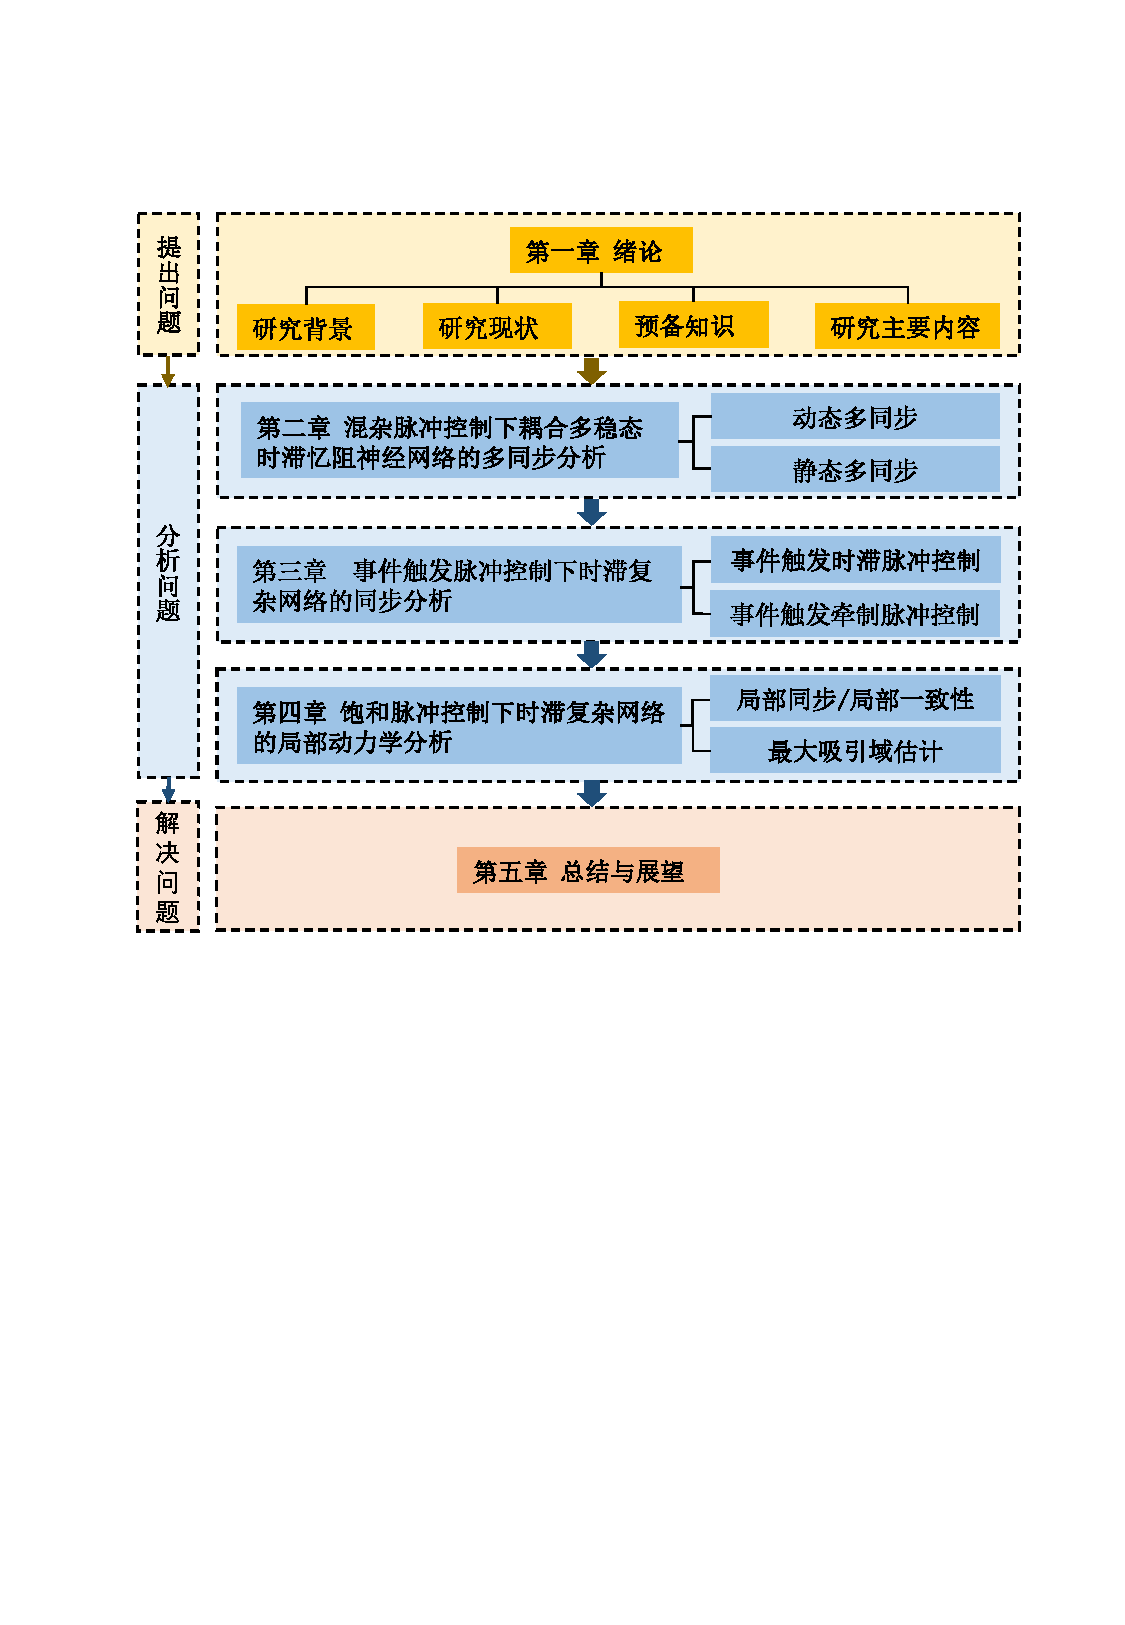
\includegraphics[scale=0.8]{./ch1Intro/fig1-1.pdf} 
    \caption{论文的结构框架 }
    \label{f1-1}
\end{figure} 
 
第一章概述了时滞复杂网络以及脉冲控制理论的研究背景和研究现状,给出了所需的代数图论和矩阵理论的相关定义与引理,并总结出主要内容和创新点。

 
第二章主要研究了在混杂脉冲控制下耦合多稳态时滞忆阻神经网络的动态多同步以及静态多同步问题,其数学模型为
    \begin{align*} 
    \begin{split}
    \dot{x}_i(t)\in&- (\check{C}+co[-\hat{C},\hat{C}]) x_i(t)+(\check{B}+co[-\hat{B},\hat{B}])f(x_i(t)) \\
    &+(\check{D}+co[-\hat{D},\hat{D}])f(x_i(t-\eta(t)))
    +\alpha\sum\limits\limits_{j=1}^{N}a_{ij}\Gamma x_j(t)+I(t)+u_i(t),
    \end{split}
    \end{align*}
和 
    \begin{align*} 
    \begin{split}
    \dot{S}(t)\in&- (\check{C}+co[-\hat{C},\hat{C}]) S(t)+(\check{B}+co[-\hat{B},\hat{B}])f(S(t)) \\
    &+(\check{D}+co[-\hat{D},\hat{D}])f(S(t-\eta(t)))+I(t).
    \end{split}
    \end{align*}
针对此网络,设计包括时滞脉冲控制和连续时间状态反馈控制的混杂脉冲控制器:
\begin{align*} 
u_i(t)=-K {\rm sign}(e_i(t))-\mu\sum\limits_{k=1}^{\infty}e_i(t-\tau(t))\delta(t-t_k),\ k\in\mathbb{Z}_+.
\end{align*}
基于状态空间划分方法和激励函数的几何特性,给出了系统具有多个局部指数稳定的周期轨道或平衡点的充分条件。然后, 利用新型的 Halanay 微分不等式和脉冲控制理论,分别获得基于 LMIs 的动态多同步以及静态多同步充分性判据。最后,给出了一个数值例子来验证所设计控制器的可行性和有效性。
 
第三章研究了事件触发脉冲控制下具有耦合时滞的复杂网络的全局同步问题。首先,分析了如下具有耦合常时滞的复杂网络的全局指数同步: 
\begin{align*} 
\dot{x}_i(t)=Bx_i(t)&+Cf (x_i(t))+c\sum\limits_{j=1}^{N}a_{ij}\Gamma x_j(t-\tau_0),\ i\in I[1,N],
\end{align*}
和 \begin{align*} 
\dot{\delta z}(t)=B\delta z(t)+Cf(\delta z(t)).
\end{align*}
设计事件触发时滞脉冲控制机制: 
\begin{align*} 
t_k=\inf \{t>t_{k-1}:\Phi (t,z(t))\leq 0\},\ k\in\mathbb{Z}_+,
\end{align*}
其中 
$\Phi (t,z(t))=e^{\alpha_k-\mu t}\big\{[e^{\mu t_{k-1}}z^T (t_{k-1})(I_N\otimes P)z(t_{k-1})]\vee (e^{\mu t_0} z^T_{t_0}(I_N\otimes P)z_{t_0})-z^T (t)(I_N\otimes P)z(t)\big\}$,此机制是将时滞脉冲控制考虑到事件触发机制中。通过构造合适的辅助函数,并利用递推法、脉冲控制理论和 Lyapunov–Razumikhin 技术,建立了基于 LMIs 的保守性更小的同步判据。

其次,进一步将牵制控制考虑到事件触发脉冲控制机制中,探讨了如下具有耦合比例时滞的基因振荡器网络的集群同步问题: 
\begin{align*} 
\begin{split}
\dot{z}_i(t)\!=\!A_vz_i(t)\!+\!B_{1v}f(z_i(t))-B_{2v}g (z_i(t))+B_2I_n
+c\sum\limits\limits_{r=1}^{\kappa}\sum\limits\limits_{j\in \mathcal{S}_r}a_{ij}\Upsilon z_j(\mu t)+u_i(t),
\end{split}
\end{align*}
和 
\begin{align*} 
\dot{w}_v(t)=A_vw_v(t)+B_{1v}f(w_v(t))-B_{2v}g (w_v(t))
+B_{2v}I_n.
\end{align*}
针对此网络,设计事件触发牵制脉冲控制器:
\begin{align*} 
u_i(t)=\left\{
\begin{aligned}
&\sum\limits\limits_{l=1}^{\infty} K_le_i(t_l)\delta (t-t_l),&i\in \mathcal{D}_v(t_l),\\
&0,&i\notin\mathcal{D}_v(t_l),
\end{aligned}
\right.
\end{align*}
其中,事件触发机制为
\begin{align*} 
t_k=\inf\{t>t_{l-1}:\  \Lambda (t)\geq 0\},
\end{align*}
这里 $\Lambda (t)=(1+ \lambda ( t-t_0))\sum\limits\limits_{v=1}^{\kappa}\sum\limits\limits_{i\in \mathcal{S}_v}e^T_i(t)Pe_i(t)-p_l\big[(1+ \lambda ( t_{l-1}-t_0))\sum\limits\limits_{v=1}^{\kappa}\sum\limits\limits_{i\in \mathcal{S}_v}e^T_i(t_{l-1})Pe_i(t_{l-1})\vee \lambda_{\max}(P)\sum\limits\limits_{v=1}^{\kappa}\sum\limits\limits_{i\in \mathcal{S}_v}\|\varphi_i\|^2_{\mu}\big]$。值得注意的是触发时刻即为脉冲时刻,其由所设计的事件触发牵制脉冲控制机制产生。并且每个集群中只有一小部分节点依据所设计的算法在触发时刻被施加脉冲控制,进一步节约了网络资源。最后,提供了数值实
例以证明所设计的事件触发机制的有效性和优越性。
 
第四章分析了分布式饱和脉冲控制下时滞复杂网络的局部动力学行为。首先,
讨论了如下具有耦合时变时滞的鲁里叶网络的局部指数同步: 
\begin{align*} 
\dot{x}_i(t)=A x_i(t)+ Bf(\tilde{D}x_i(t)) +c\sum\limits_{j=1}^N \omega_{ij}\varGamma x_j(t-q (t))+\mathcal{U}_i(t),\ i\in I[1,N].
\end{align*}
针对此网络,设计如下具有执行器饱和的分布式脉冲控制输入:
\begin{align*} 
\mathcal{U}_i(t)=\sum\limits_{l=1}^{\infty}{\rm sat}(u_i(t)) \delta(t-t_l),\ l\in\mathbb{Z}_+,
\end{align*} 
其中
$
u_i(t)=K \sum\limits\limits_{j\in \mathcal{N}_i}^{N}a_{ij}(x_j(t)-x_i(t))
$。 利用反证法、脉冲系统的比较原理和平均脉冲区间的方法,得到了不依赖于时滞的基于 BMIs 的局部同步判据。为了降低保守性,选取最新的具有更多松弛变量的改进凸包表示法来处理分布式饱和的脉冲项,并且开发了一种与收缩不变集完全不同的估计吸引域方法。

其次,研究了分布式饱和脉冲控制下如下具有切换拓扑的非线性时滞多智能体系统的局部一致性:
\begin{align*} 
\left\{\begin{aligned} 
\dot{x}_0(t)=&Ax_0(t)+Bf(x_0(t-\tau(t))),\\
\dot{x}_i(t)=&Ax_i(t)+Bf(x_i(t-\tau(t)))+u_i(t).
\end{aligned}\right.
\end{align*}
设计分布式饱和脉冲控制器:
\begin{align*} 
u_i(t)=\sum\limits_{k=1}^{\infty}{\rm sat}(w_i(t)) \delta (t-t_k),\ k\in\mathbb{Z}_+,
\end{align*}
其中 $
\omega_i(t)=F\big(\sum\limits_{j\in \mathcal{N}_i}a^{\sigma(t)}_{ij}(x_j(t)-x_i(t))+b^{\sigma(t)}_i(x_0(t)-x_i(t))\big) 
$。利用反证法、Lyapunov-Razumikhin 技术,建立起相应的局部一致性判据。通过构造依赖于脉冲时刻的复合的 Lyapunov 函数,进一步降低了受控系统的保守性。为了估计出最大的吸引域,通过适当的矩阵变换,建立起基于 LMIs 的优化问题,并通过 Matlab 软件中的 Yalmip 工具箱求解相应的最大吸引域的数值解。最后,通过数值实例验证了所提理论结果的有效性和优越性。
 
第五章总结了全文的主要内容,并对未来的研究工作进行展望。


\subsection{主要创新点}
本文通过设计不同类型的脉冲控制,对时滞复杂网络的多种动力学行为进行了全面分析:通过设计混杂脉冲控制器,实现了耦合多稳态时滞忆阻神经网络的动态多同步以及静态多同步,脉冲控制中时变时滞的上界小于脉冲间隔的限制被取消, 降低了结果的保守性。此外,设计了两种依赖于 Lyapunov 函数的事件触发脉冲控制协议,分别获得了时滞复杂网络不依赖于时滞的全局指数同步和集群同步判据,降低了不必要的网络资源的浪费。最后,通过设计分布式的饱和脉冲控制,对时滞复杂网络的局部动力学进行分析,并开发了一种全新的估计吸引域的方法,通过建立相关的优化问题估计出最大的吸引域。

文中结果是对现有一些结果的丰富和扩展,主要创新点具体如下:

\textbf{1. 探索了耦合多稳态时滞忆阻神经网络的多同步问题,设计了由时滞脉冲控制和连续时间状态反馈控制构成的混杂脉冲控制器,分别给出了动态多同步和静态多同步的充分性判据。文中讨论了脉冲控制中时变时滞存在的情况,取消了脉冲控制中时变时滞的上界小于任意脉冲区间的限制,进一步降低了结果的保守性。}

在已有的耦合时滞忆阻神经网络中,通常存在一个唯一的平衡态 (平衡点或周期轨道或混沌吸引子)。为了提高神经网络的储存能力,基于状态空间划分方法和激励函数多分段的几何性质,给出了系统具有多个局部指数稳定的周期轨道或平衡点的充分条件。其次,在现有的多同步文章中,脉冲控制器没有考虑时滞的影响。为此,设计了一种由时滞脉冲控制和连续时间状态反馈控制组成的新型混杂脉冲控制器,再利用改进的 Halanay 不等式技术、微分包含以及脉冲控制理论,分别获得了耦合多稳态时滞忆阻神经网络的动态多同步和静态多同步的充分性判据。 值得注意的是,系统的状态时变时滞可微的限制和脉冲控制中的时变时滞的上界小于任意脉冲区间的要求都被已取消,即允许时滞区间中可能存在多个脉冲。

\textbf{2. 讨论了具有耦合常时滞的复杂网络的全局指数同步问题,设计了基于 Lyapunov 函数的事件触发时滞脉冲控制协议,给出了全局指数同步判据。其中, 取消了对 Lyapunov 函数单调性的限制,进一步降低了结果的保守性。}

已有的脉冲控制大多都是基于时间触发来进行信息传输和控制更新,为了减少不必要的网络资源的浪费和提高控制效率,将时滞脉冲控制与事件触发机制相结合,设计了新型的基于 Lyapunov 函数的事件触发时滞脉冲控制协议,极大地减少控制成本,增加系统的鲁棒性,避免了控制冗余。通过构造合适的辅助函数并利用 Lyapunov-Razumikhin 技术和递推法,得到了不依赖于时滞的时滞复杂网络的全局指数同步判据。
一般来说, Lyapunov 函数要求在触发的时间间隔内严格单调递减,以确保触发时间序列是无穷的。文中放弃了这一限制,允许 Lyapunov 能量函数在下一个触发瞬间之前是递增,并能保证在有限的触发次数下实现同步。最后,验证时滞复杂网络在所设计的事件触发时滞脉冲控制下能够有效地避免芝诺现象。

 

\textbf{3.  针对具有耦合比例时滞的基因振荡器网络集群同步问题,建立起事件触发牵制脉冲控制机制,给出了集群同步判据。通过设计合适的算法,每个集群中只有一小部分节点在触发时刻被施加脉冲控制,进一步降低了控制成本。}

进一步将事件触发脉冲控制机制推广到具有比例时滞的脉冲泛函微分方程,提出了新型的依赖于 Lyapunov 函数的事件触发脉冲控制机制。其中,触发时刻由所设计的事件触发机制产生,触发时刻即为脉冲时刻。目前已经存在的事件触发脉冲控制都是对大规模网络中所有的节点施加控制,从而导致网络具有较高的能耗。为了解决这一问题,进一步将牵制控制考虑到所建立的事件触发脉冲控制机制中,设计了事件触发牵制脉冲控制协议,解决了具有耦合比例时滞的基因振荡器网络集群同步问题,并给出了基于 LMIs 的 集群同步判据。通过设计合适的算法,每个集群中只有一小部分节点在触发时刻被施加脉冲控制。 与已有的事件触发牵制控制不同,所设计的事件触发牵制脉冲控制仅在触发时刻瞬时改变网络中部分节点的状态,而在非触发的脉冲时刻不再施加任何控制,并且消除了芝诺行为。


\textbf{4. 针对具有耦合时变时滞的有向鲁里叶网络,研究了分布式饱和脉冲控制下的局部指数同步和吸引域估计问题。开发了全新的吸引域的估计方法并建立优化问题分别给出吸引域和平均脉冲区间的最大估计。}

目前,由于脉冲饱和项难处理以及吸引域难于估计,关于饱和脉冲控制下时滞复杂网络的研究工作甚少,尚处于起步阶段。通过采用最新改进的饱和函数凸包表示来处理饱和脉冲约束项,并利用反证法、脉冲系统的比较原理以及平均脉冲区间方法,给出了具有耦合时变时滞的鲁里叶网络的局部指数同步判据并建立优化问题估计出最大的吸引域。目前,已有的关于饱和脉冲的结果基本上都是借助于收缩不变集来估计吸引域,这要求 Lyapunov 函数在此集合中的任意非零点上是严格单调递减的。本文取消了这一限制,开发了一种保守性更小的估计吸引域的方法。其次,
由于耦合的时变时滞的上界与局部同步判据无关,仅与收敛指数有关,因此,时滞的上界小于某个常数的限制被取消,使得所得结果保守性更小。最后,只要平均脉冲区间满足一定条件,不再对脉冲间隔的上下界有任何限制,这意味着允许非均匀分布脉冲信号的存在。



\textbf{5. 通过设计分布式饱和脉冲控制协议,讨论了具有切换拓扑的非线性时滞多智能体的局部一致性。构造了一种全新的依赖于脉冲时刻的复合型 Lyapunov 函数,以获得最大的吸引域估计。}

已有的一致性结果主要集中在全局一致性上,本文讨论了具有执行器饱和切换拓扑的非线性时滞多智能体系统的局部一致性问题,
利用 Lyapunov-Razumikhin 技术和反证法,得到了不依赖于时滞的局部一致性判据并给出了最大吸引域的估计。由于结构简单,目前存在的结果大多数都是基于一般的二次  Lyapunov 函数。然而,利用二次 Lyapunov 函数估计出的吸引域与真实的吸引域之间存在较大差距。为了降低由二次 Lyapunov 函数带来的保守性,通过构造了一个具有更多辅助矩阵的复合的依赖于脉冲时刻的 Lyapunov 函数,并采用了一种具有更多可用的松弛变量的改进的凸包表示法,在最大程度上降低了保守性,使得所估计的吸引域更接近真实吸引域。 

 

本文部分结果发表在~Neural Networks,IEEE Transactions on Cybernetics,IEEE Transactions on Neural Networks and Learning Systems~等国际刊物上,部分结果已投稿至~IEEE
Transactions on Automatic Control,IEEE Transactions on Systems, Man, and Cybernetics: Systems~等期刊。具体详见作者发表论文的清单。
